\phantomsection
\chapter{Face detection}

\noindent Face detection is the first step following image acquisition, and is compulsory for facial expression recognition. At the end of this step, only useful information will remain. It will not only reduce processing time during the feature extraction step, but will also improve the classifier by discarding useless information.
\newline

\phantomsection
\section{Detection}

\vspace{\baselineskip}
\noindent Detection is finding out if the input image or video sequence represents or contains a particular object, usually followed by recognition. In our system, facial expression recognition will be performed. However, depending on the recognition, an additional tracking step can be needed. Tracking consists in following a moving target along the images of a video sequence \cite{DIN08}.
\newline

\noindent An object detector can be defined as a "black box" taking an image as input. Its input depends on the type of detector, whether it is high level or low level. At a high level the output can be considered as an annotated image saying where the object of interest appears \cite{DIN08}. For example, the output can look like Figure~\ref{output_example_face_detection} \cite{DIN08}.
\newline

\begin{figure}[!h]
\begin{center}
\noindent 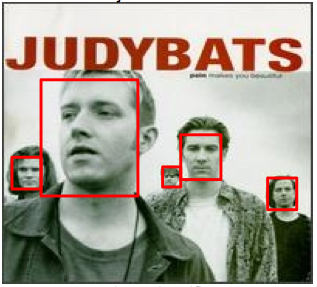
\includegraphics[scale=0.7]{figures/output_example_face_detection} 
\newline
\caption{Example of an output of face detection \cite{DIN08}}
\label{output_example_face_detection}
\end{center} 
\end{figure}

\noindent At a low level, the output is not an annotated image anymore. The core of the object detector is a basic component saying if an instance of the object of interest is contained in a certain region or sub-region of the original image. This kind of detection is performed by a binary classifier \cite{DIN08}. There is an example of a binary classifier output in Figure~\ref{output_example_face_detection_binary_classifier} \cite{DIN08}.
\newline

\begin{figure}[!h]
\begin{center}
\noindent 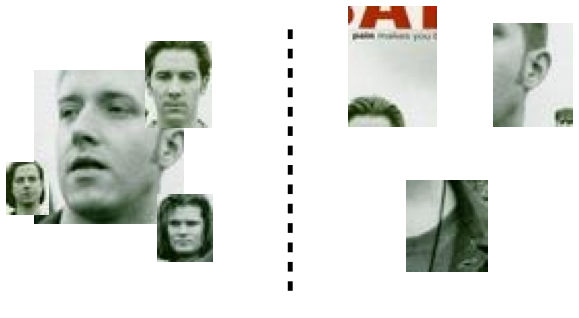
\includegraphics[scale=0.5]{figures/output_example_face_detection_binary_classifier} 
\newline
\caption{Example of a binary classifier output for face detection}
\label{output_example_face_detection_binary_classifier}
\end{center} 
\end{figure}

\phantomsection
\section{Classifiers}

\vspace{\baselineskip}
\noindent Classification aims to solve the problem of identifying in a set of categories or sub-populations to which a new observation belongs. It is based on a training set of data that contains instances whose category affiliations are known. Data can be labeled based on some measures of inherent similarity; for example, vectors representing the distance between instances \cite{CLASS}.
\newline









